%%
%% This is file `sample-sigconf.tex',
%% generated with the docstrip utility.
%%
%% The original source files were:
%%
%% samples.dtx  (with options: `sigconf')
%% 
%% IMPORTANT NOTICE:
%% 
%% For the copyright see the source file.
%% 
%% Any modified versions of this file must be renamed
%% with new filenames distinct from sample-sigconf.tex.
%% 
%% For distribution of the original source see the terms
%% for copying and modification in the file samples.dtx.
%% 
%% This generated file may be distributed as long as the
%% original source files, as listed above, are part of the
%% same distribution. (The sources need not necessarily be
%% in the same archive or directory.)
%%
%% The first command in your LaTeX source must be the \documentclass command.
\documentclass[sigconf,authordraft]{acmart}
%%%% As of March 2017, [siggraph] is no longer used. Please use sigconf (above) for SIGGRAPH conferences.

%%%% Proceedings format for SIGPLAN conferences 
% \documentclass[sigplan, anonymous, review]{acmart}

%%%% Proceedings format for SIGCHI conferences
% \documentclass[sigchi, review]{acmart}

%%%% To use the SIGCHI extended abstract template, please visit
% https://www.overleaf.com/read/zzzfqvkmrfzn

%%
%% \BibTeX command to typeset BibTeX logo in the docs
\AtBeginDocument{%
  \providecommand\BibTeX{{%
    \normalfont B\kern-0.5em{\scshape i\kern-0.25em b}\kern-0.8em\TeX}}}

%% Rights management information.  This information is sent to you
%% when you complete the rights form.  These commands have SAMPLE
%% values in them; it is your responsibility as an author to replace
%% the commands and values with those provided to you when you
%% complete the rights form.
\setcopyright{acmcopyright}
\copyrightyear{2020}
\acmYear{2020}
\acmDOI{10.1145/1122445.1122456}

%% These commands are for a PROCEEDINGS abstract or paper.
\acmConference[Automated Software Engineering '20]{Automated Software Engineering (ASE 2020)}{June 03--05, 2018}{Woodstock, NY}
\acmBooktitle{Automated Software Engineering (ASE 2020)}
\acmPrice{15.00}
\acmISBN{978-1-4503-XXXX-X/18/06}


%%
%% Submission ID.
%% Use this when submitting an article to a sponsored event. You'll
%% receive a unique submission ID from the organizers
%% of the event, and this ID should be used as the parameter to this command.
%%\acmSubmissionID{123-A56-BU3}

%%
%% The majority of ACM publications use numbered citations and
%% references.  The command \citestyle{authoryear} switches to the
%% "author year" style.
%%
%% If you are preparing content for an event
%% sponsored by ACM SIGGRAPH, you must use the "author year" style of
%% citations and references.
%% Uncommenting
%% the next command will enable that style.
%%\citestyle{acmauthoryear}
\usepackage{algorithm}
\usepackage{algorithmic}
%%
%% end of the preamble, start of the body of the document source.
\begin{document}

%%
%% The "title" command has an optional parameter,
%% allowing the author to define a "short title" to be used in page headers.
\title{Metamorphic Services to Automatically Learn when to Retrain Deep Neural Networks}

%%
%% The "author" command and its associated commands are used to define
%% the authors and their affiliations.
%% Of note is the shared affiliation of the first two authors, and the
%% "authornote" and "authornotemark" commands
%% used to denote shared contribution to the research.
\author{Hemanth Gudaparthi}
%%\authornote{Both authors contributed equally to this research.}
\authornotemark[1]
\affiliation{%
  \institution{University of Cincinnati}
  \streetaddress{2600 Clifton Ave.}
  \city{Cincinnati}
  \state{Ohio}
  \postcode{45220}
}
\email{gudapahh@mail.uc.edu}

\author{Reese Johnson}
\affiliation{%
  \institution{Metropolitan Sewer District of Greater Cincinnati}
  \streetaddress{1 Th{\o}rv{\"a}ld Circle}
  \city{Cincinnati}
  \state{Ohio}
  }
\email{reese.johnson@cincinnati-oh.gov}

\author{Nan Niu}
\affiliation{%
 \institution{University of Cincinnati}
 %%\streetaddress{Rono-Hills}
 \city{Cincinnati}
 \state{Ohio}}
\email{nan.niu@uc.edu}
 
%%
%%
%% By default, the full list of authors will be used in the page
%% headers. Often, this list is too long, and will overlap
%% other information printed in the page headers. This command allows
%% the author to define a more concise list
%% of authors' names for this purpose.
\renewcommand{\shortauthors}{H. Gudaparthi, et al.}

%%
%% The abstract is a short summary of the work to be presented in the
%% article.
\begin{abstract}
   We then have to retrain them either with new data or new methods to improve the training accuracy. There are many studies on how to retrain, how much or what kind of training data would be good for retraining. We in this paper provide a novel metamorphic service which will help in understanding when to retrain the neural network. There are different kind of deep learning methods but we are particularly interested in Recurrent Neural Networks (RNNs) as they are best suitable for time series data. In the results we show that the metamorphic service will give a threshold value of when to retrain will not only consider to keep accuracy measure intact but also considers robustness of the deep learning algorithm. We also provide results to show that the deep learning algorithm's robustness is maintained using a metamorphic relation we have discovered in our previous paper.
  % We will present in the results section showing when to retrain.
\end{abstract}

%%
%% The code below is generated by the t9ol at http://dl.acm.org/ccs.cfm.
%% Please copy and paste the code instead of the example below.
%%
\begin{CCSXML}
<ccs2012>
 <concept>
  <concept_id>10010520.10010553.10010562</concept_id>
  <concept_desc>Computer systems organization~Embedded systems</concept_desc>
  <concept_significance>500</concept_significance>
 </concept>
 <concept>
  <concept_id>10010520.10010575.10010755</concept_id>
  <concept_desc>Computer systems organization~Redundancy</concept_desc>
  <concept_significance>300</concept_significance>
 </concept>
 <concept>
  <concept_id>10010520.10010553.10010554</concept_id>
  <concept_desc>Computer systems organization~Robotics</concept_desc>
  <concept_significance>100</concept_significance>
 </concept>
 <concept>
  <concept_id>10003033.10003083.10003095</concept_id>
  <concept_desc>Networks~Network reliability</concept_desc>
  <concept_significance>100</concept_significance>
 </concept>
</ccs2012>
\end{CCSXML}

\ccsdesc[500]{Computer systems organization~Embedded systems}
\ccsdesc[300]{Computer systems organization~Redundancy}
\ccsdesc{Computer systems organization~Robotics}
\ccsdesc[100]{Networks~Network reliability}

%%
%% Keywords. The author(s) should pick words that accurately describe
%% the work being presented. Separate the keywords with commas.

\keywords{retraining, recurrent neural networks, metamorphic relations}

%% A "teaser" image appears between the author and affiliation
%% information and the body of the document, and typically spans the
%% page.

%%
%% This command processes the author and affiliation and title
%% information and builds the first part of the formatted document.
\maketitle

\section{Introduction}
Deep Neural Networks (DNNs) are being widely used in different applications lately. Manual software implementations have be taken over by this automated learning machines. DNNs are being used in various fields such as natural language processing, computer games, weather prediction, and even in software engineering field for code generation, bug fixing, etc. These DNNs have the promise of giving you better/best of the results compared to other machine learning algorithms which has been evident in recent years. But the problem with DNNs is that with time they turn out to show significant reduction in accuracy due to different reasons like new data in the stream, having adversarial data points, reduction in neuron coverage, etc.[cite apricot, adversarial examples [14] in apricot, [59] in apricot].
 
 Before deployment Deep Neural Networks are trained on large amounts of data which contains training, validation and test datasets (as shown in Fig 1). Each of this training dataset has a predefined label or an expected output that DNNs should be able to predict at the end of training. Then we need a test dataset for testing how good DNNs are trained. DNNs will take each test data point (test case) as input and have to predict the actual label of that test sample. If the result of DNNs are inconsistent from the actual result we consider that as failed case. Once the system is trained and tested well it will be deployed to perform the prediction or classification accordingly. Since these DNNs are static and can only remember the data they have trained on it is difficult for them to adapt to new data (unseen data). Particularly when we are talking about time-series data (e.g. weather data) it is hard to know when the system will turn out to be inaccurate. 
 
Particularly with Metropolitan Sewer District of Greater Cincinnati's (MSDGC's) combined sewer overflow (CSO) data, there will be lot at stake because of inaccurate and not robust enough. reused.Combined sewer systems manage the storm water runoff, sewage, and industrial wastewater in a single pipe.During heavy rainfalls or other events these pipes will reach their maximum capacity. When they exceed this limit overflow or combined sewer overflow (CSO) occurs that results in draining untreated water in to nearby water bodies [7][Cite our paper]. We can predict these overflow situations using DNNs which is not a trivial thing. Stakeholders like in MSDGC will have very less idea of if or when to reapair the DNNS. With a lot of life and unhealthiness at stake, it is not preferable to \emph{not} know when the system has to be diagnosed for being imprecise and not so robust during prediction.

%\usepackage{subcaption}
%\usepackage{graphicx} % omit 'demo' for real document
\begin{figure*}
\includegraphics[width = 6in]{Pre-Deployment.png}
\caption{Figure showing the training of RNN in pre-deployment phase to adjust the weights of the network } \label{fig:1}
\end{figure*}

 
Various research studies have been conducted on how to handle the inaccuracy or the mis-classifications of DNNs but there are very few [apricot, few on the laptop] studies that concentrate on when to know that DNNs needed to be 'repaired'. Some of the studies done based on accuracy of the models [apricot]. They consider change in accuracy measure as the correct time to retrain the model.Particularly [Apricot] shows that their method improves test accuracy by an average of 1.19\%  on Convolutional Neural Networks (CNNs) and an average of 0.895\% in ResNet models. Some of the researchers have also considered similarity scores between new and old data to incrementally train DNNs. Most of them will consider loss functions (mean square loss, mean logrithmic loss, etc.) to evaluate the failure of DNNs.  %EXPLAIN ABOUT FIG 1 AND HOW PREDEPLOYMENT PHASE IS USED IN HERE

But the problem with these models is that the performance of DNNs are mostly judged over by the training accuracy (accuracy of DNNs during training) and testing accuracy (accuracy of DNNs while predicting on test cases). These are easy to apply before deployment but post deployment it is difficult for stakeholders to understand the concept of accuracy or when will be the correct time to retrain. Consider change in accuracy from 89 - 85\%. It is hard to judge by this change to know that if it is the right time to repair DNN. We in this study present you a novel metamorphic service which could automatically detect and let the stakeholders know the exact time at which DNNs should be diagnosed or repaired. Accuracy is defined as the proximity of measurement of predicted values to true values (e.g. For labels 0, DNN's prediction could be 0.2 which means DNN is 80\% accurate). Since accuracy is not a very good measure when it comes to stressful conditions or while predicting on new stream of data we also consider the robustness of DNN to show that at a particular time 't' DNN will not accurate and robust enough to continue. We will also show the robustness measure of the RNNs until the point of repair (i.e. time 't') with changing window sizes of gradients to measure robustness.%Using the 'how to repair' techniques[apricot, etc.] before or after the resultant time of this research would overfit or underfit the weights of neurons and cause in reduction of performance than improving it. %A robust DNN can perform well in adversarial conditions, can adjust to the unseen data, and perform better in stressful environments. This will help the stakeholders in understanding and diagnosing the DNNs using aforementioned techniques [apricot, other examples]
 

 
We consider RNNs as our deep learning models in this research as they are known to be the best when it comes to time-series data[CITE 5 in ICSE'S]. In our previous paper we have explored how robust recurrent neural networks are in adversarial conditions like missing data from sensors [CITE US]. RNN has internal states that helps in processing time-series data. They will have a cell which will remember the important information from historical data and restructure its internal state (weights of neuron connections) with every incoming new data sample. This restructuring the weights in RNNs is called as backpropagation which can be seen in Fig 2. We use this weights to help us know the robustness measure of the RNN. %Explain about RNNs

Main contributions of our research are:
\begin{itemize}
  \item We present a novel metamorphic service which could help in automatically detecting the exact time for the RNNs to be diagnosed or repaired post deployment.
  \item We also show that by considering varying window size of the change of weights during backpropagation would help in getting more robust, accurate RNN which also takes longer time to fail (to get repaired). We automated this 
  \item Our metamorphic service can be applied on any variant of RNNs  which are used in time series prediction. %Remove DNNs or other kind of DNNs (CNNs, ResNet, etc.)
\end{itemize}



\section{Background}
Repairing of RNNs before deployment has been done by many researchers. These techniques involve retraining, adjusting weights, etc. By these studies we can see that even post deployment DNNs can get inaccurate due to different causes (such as new data, change of weights due to backpropagation, etc.). In [APRICOT, Incremental Learning] paper they mention how DNNs are inherently imprecise and their inability to adjust weights on new data. RNNs in particular are very good dealing with new data as they remember the information from historical time series as well as learn new weight adjustments with incoming data.[recurrent neural networks for time series classification]. RNNs are also being used for weather prediction, overflow prediction recently by researchers [our paper Zhang et al., search for weather part]. RNN models have promising results to be better at time series predictions.

\subsection{Recurrent Neural Networks}


% GRADIENT DESCENT. HOW WEIGHTS ARE CHANGED, ETC.



 RNN has three layers which are called input layer, hidden layer, and output layer. As we can see from Figure 2, RNN will takes input at a particular time 't-1' which is called inp (t-1) and using the hidden layer \emph{h}, they do some non-linear transformation to produce output Out (t-1). When this output is compared with the ground truth label at inp (t), change of weights in the neurons is known by knowing the distance between true value and predicted value. inp(t-1), inp (t), inp (t+1), Out (t-1), Out (t), Out (t+1) are inputs and outputs of RNN at times 't-1', 't', and 't+1' respectively and \begin{math}\Delta \end{math} w is the change of weights due to backpropagation. The change of weights \begin{math}\Delta \end{math} w is based on the error rate (inaccuracy) from predicted to ground truth.
 
RNN also have different variations like Long Short Term Memory (LSTM), Gated Recurrent Unit (GRU), Independently Recurrent Neural Network (Ind RNN), etc. All these variations have some architectural differences like LSTM has three gates (input gate, ouput gate, forget gate), while GRU has two main gates (input gate, output gate) and there is reset state, and Ind RNN does not have any gates. Ind RNN operates on the neuron level by using parallel connection for each feature. But all these variations of RNNs have common working operation (as shown in Figure 2). All these RNNs as they go forward in time, RNN learns more and more about the kind of data. So as RNN trains with incoming data there will be a gradient descent in the \begin{math}\Delta \end{math} w which means accuracy will increase gradually with the incoming data and backpropagation.
 
%SPEAK ABOUT RNNS USE IN MSDGC WHY ROBUSTNESS IS IMPORTANT

Particularly in the paper [Apricot], authors argue that the DNNs are to be 'repaired' if the model is not accurate enough. Their research is concentrated on pre-deployment phase of DNNs where they try to achieve higher accuracy by weight adaptation technique. The main contribution of their research result is stated as increasing average accuracy of the CNN models by 1.19\% and ResNet models by 0.895\%. But when they claim to 'repair' the DNNs while they are not accurate enough they have not mentioned which percentage of accuracy is not accurate enough. We concentrate on this point to further our investigation to know when these software solutions such as RNNs are considered to be 'repaired'. Please note that we are not providing any method to repair the RNNs but providing a research result to know when they are to be 'repaired'. 


\subsection{Gradient Descent}

Gradient descent algorithm is an optimization function which finds local minimum in the loss function. After calculating error function (distance between predicted (t) to true (t)) after each time step the error function should be reduced for the algorithm to reduce the error and increase the accuracy. In equation (1), \begin{math}\theta_i\end{math} is the error function, \begin{math}\alpha\end{math} is the learning rate. The error function theta is reduced by subtracting the derivative of error produced after each time step. \begin{math}J(\theta) \end{math} is the mean squared error function, where m is the number of time steps processed until now. For example, if RNN is processing inp(t+3), then m will be 3 (which are inp(t), inp(t+1), inp(t+2)). Here, \begin{math}h_\theta(X_i)\end{math} is the prediction at \begin{math}
 X_i\end{math} and \begin{math} y_i \end{math}  is the ground truth at time step 'i'.
% m is number of time steps seen until this point in time. for example if the rnn is taking inp(t+3), m would be t-1, t, t+1, t+2
y\_i
\begin{equation}
  \theta_i = \theta_i - \alpha*\frac{\partial}{\partial \theta_i}*J(\theta)
\end{equation}

\begin{equation}
J(\theta) = 1/2m \sum_{i=1}^{m} [h_\theta(X_i) - y_i]^2
\end{equation}


\begin{figure}
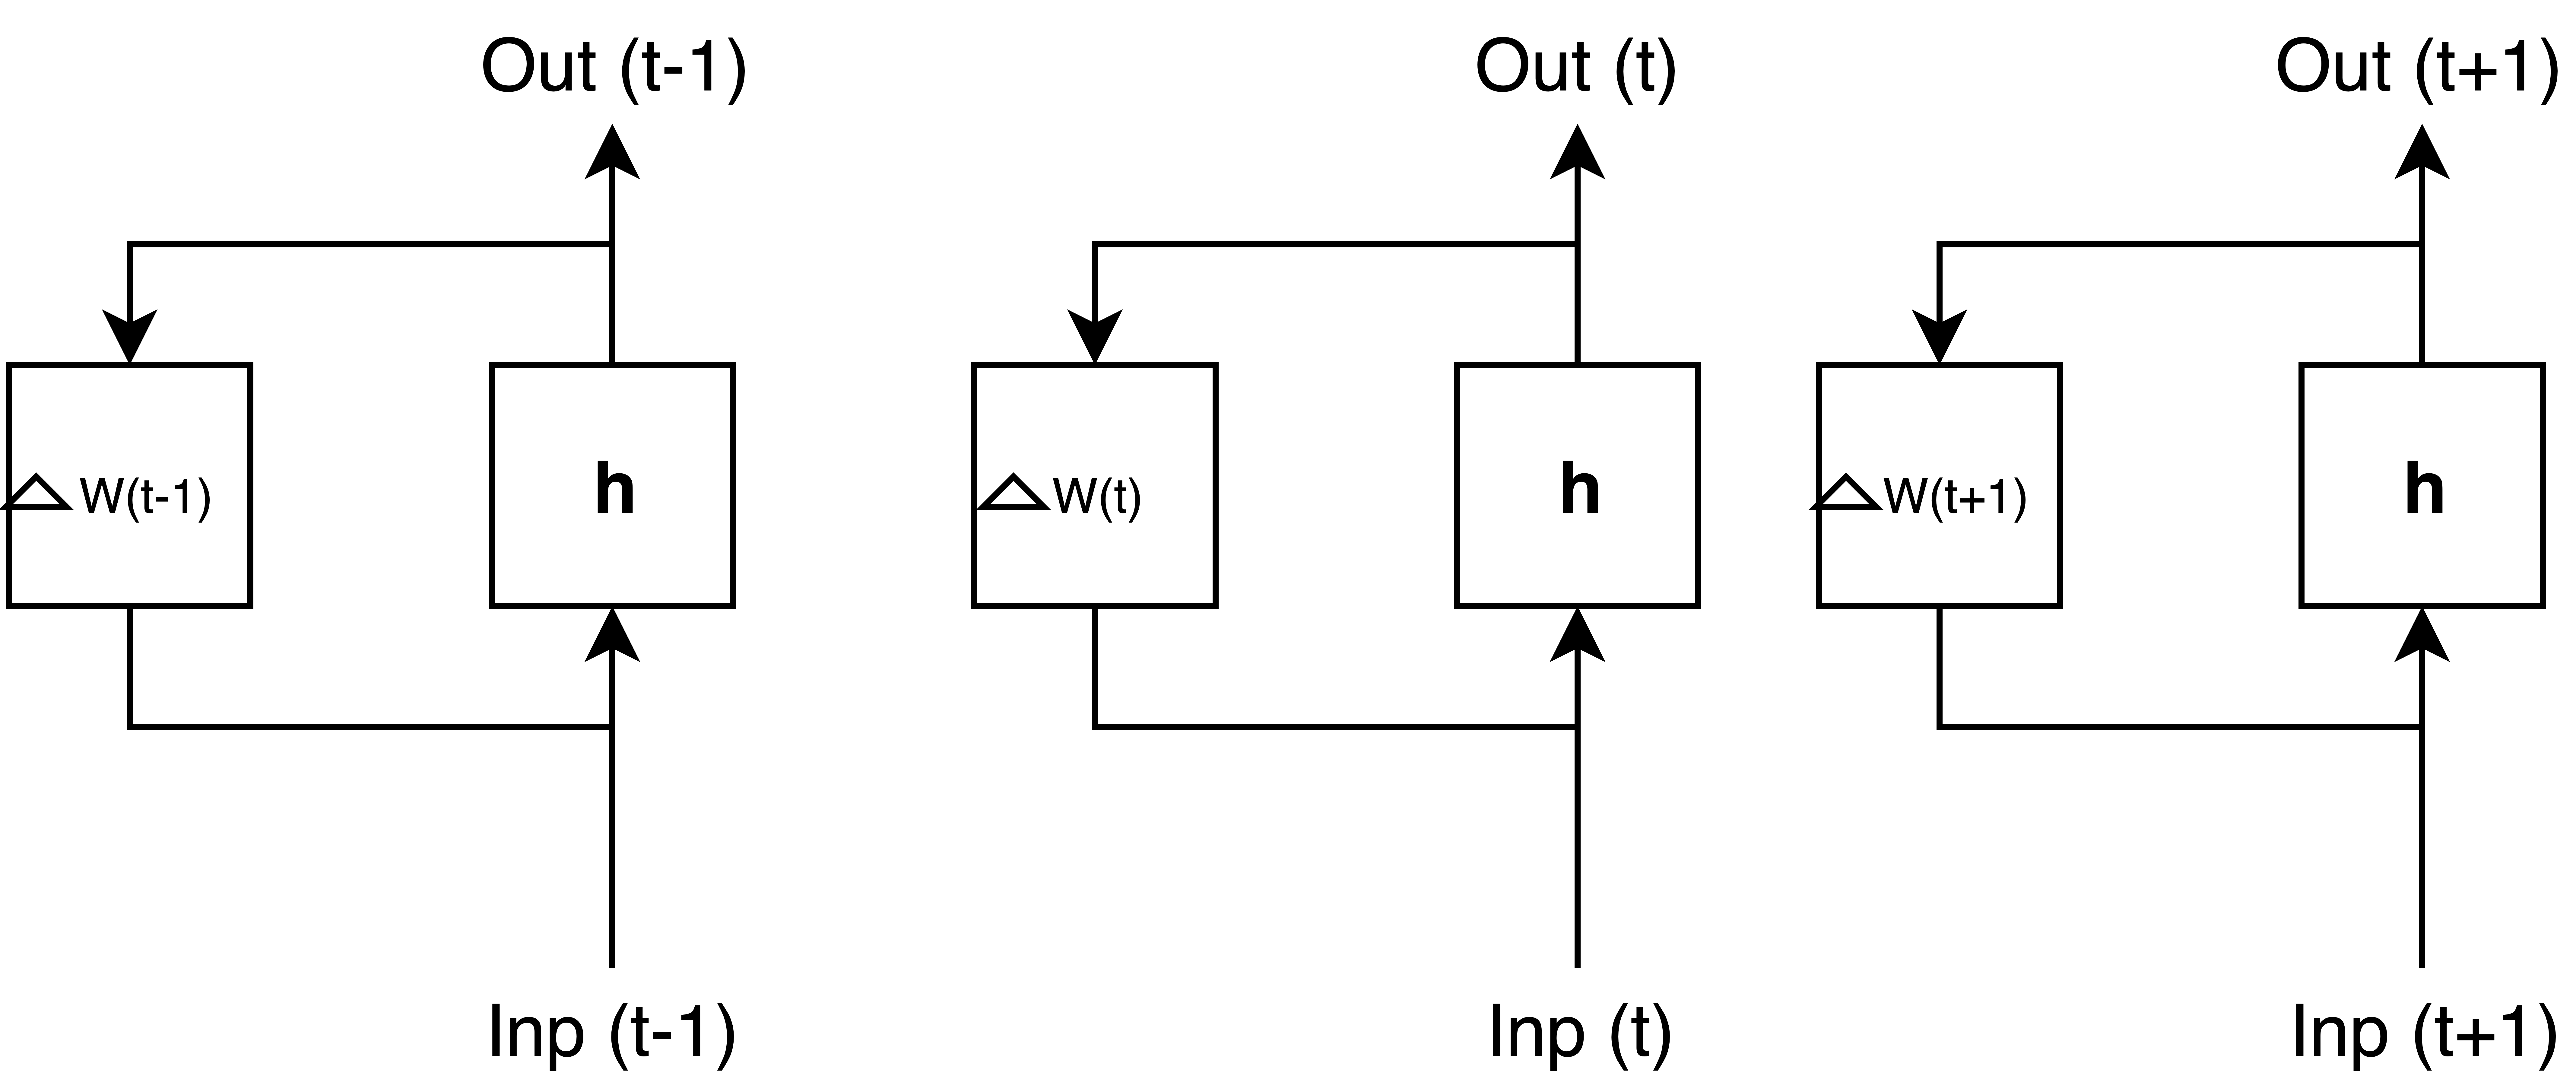
\includegraphics[width=\linewidth, scale = 0.5]{RNN_background.png}
\caption{Figure showing the change of wieghts in RNN while training on time series data.} \label{fig:1}
\end{figure}


\section{Data}
\begin{table}%[t]
  \caption{Snippet of CSO data used for experimentation}
  \label{tab:freq}
 \begin{tabular}{||c c c c c c||} 
    \toprule
    Day &Time& Flow (mgd)&Velocity (ft/sec)&Level (ft)&Overflow\\
     \midrule
     : & : & : &: & : &:\\
    August 18 &10:00 & 2.5 &0.70 & 540.2 & 1\\
    August 18 &10:05 & 10.3 &0.09 & 547.2 & 9\\
    August 18 &10:10 & 6.1 &0.18 & 543.2 & 4\\
    August 18 &10:15 & 4.2 &0.39 & 541.2 & 2\\
    : & : & : &: & : &:\\
  \bottomrule
\end{tabular}
\end{table}

We are using the same CSO data that was used in our previous paper [CITE our paper]. This CSO data contains 6 columns as shown in the Table 1. It contains data from August 18, 2017 to September 6, 2018. All the data is collected from sensors at an 5 minutes interval. Each column other than data and time are collected from the respective sensors. Here Flow column represents the amount of water flown (in millions of gallons per day) through the sewer pipes at that particular interval of time. If the flow levels are higher then we might infer that the capacity of the pipes would not be enough to handle any more water and hence there might be an overflow.

Velocity column in the table represents the velocity of the water flowing through the pipes (in feet per second). This velocity of the water is controlled by a gate which is raised to certain level to allow some water to overflow into the river. Higher velocity with higher values of flow will have a certainty of resulting in overflow. Level column represents the elevation of water in the trunk sewer collected from different manholes and households. If the value of this level exceeds 546.58 ft then it means that sewer is overflowing.

The overflow status given here contains 8 sub-categories:
\begin{itemize}
  \item \emph{Label 1:} There is a normal flow in the pipes 
  \item \emph{Label 2-5:} Sensors are experiencing different levels of elevated water flow from these pipes
  \item \emph{Label 6:} There has been an overflow without any rainfall. This can occur due to heavy usage of sewers or if the water purifying facility has reached its maximum limit. If the purifying facility reaches maximum limit they tend to send the extra water through overflow pipes. 
  \item \emph{Label 7:} There has been an overflow with heavy rainfall. Whenever there is heavy rainfall the water from different manholes will raise the water elevation in sewer pipes.
  \item \emph{Label 8:} The sensor data or the overflow pipes are not being used at this point of time. There are various areas where these overflow pipes are located to overflow excessive water into different parts of the Ohio river. So one of the pipes coming from a locality may not experience overflow. This label represent the status of that particular area.
  \item \emph{Label 9:} Overflow pipes are being flooded with the incoming streams of water. 
\end{itemize}



\section{Methodology}

\subsection{Pre-Deployment}
Firstly, we take 25000 samples of roughly 50,000 data samples for training, validating, testing RNNs as shown in Figure 1 (pre-deployment phase). We divide these 25000 samples into 60\%, 20\%, 20\% splits for training data, validation data and testing data respectively. We have considered three different variation of RNNs as specified in this paper, LSTM, GRU, and Ind RNN to show that our approach will work on different variants of RNNs. We train our RNNs in such a way that it has to predict the overflow label of next time step when given attributes of current time step. For example, from Table 1, if we have given input of Flow, Velocity, Level at time step 10:00 on August 18, then the RNNs output should be '9' which is the overflow value at time stamp 10:05 on August 18.
%speak about figure 1 clearly.

As we can see from Figure 1, we input the time series data into a RNN which is not trained (weights will be randomly initialized). As the training starts the model weights are adjusted to the kind of data it is getting in. Once the RNN learns to see the patterns in the data then the learned weights of RNN will be perfect in predicting the data. We made sure to use early stopping method which stops early before the completion of epochs (iterations) in the training phase. This helps in prevention of overfitting. During the training phase RNN will also validate to see if the learned weights are only good on the data it is trained on or if it can be used on unseen data. During testing, RNN ability to predict on unseen samples is tested. If the predictions are accurate enough then we can say that the weights of RNNs are adjusted very well on the data. After this phase generally a RNN is ready for deployment.%write about testing data. And deployment. accuracies achieved by the model can be given in results. DONT WRITE THE ACCURACIES IN HERE.

Table 2 shows the structure of all variants of RNNs used in experimentation. We have used 1 Input, 3 hidden, and 1 output layer for training the RNNs. For all the layers (except the output layer) we have used 128 neurons each. The one neuron in the output layer is used to predict the overflow value at the next time step (overflow at 't+1', while input is at time 't'). Input layer has shape of (17,500 $\times$ 3) which is the training data (70\% of 25000) samples. This network is fully connected (i.e. all the neurons are connected to every other neuron in feedforward as well as feedback way)

We have used activation function called rectified linear unit (ReLu) for all the layers except the output layer. This is the most common kind of activation function used in neural networks. ReLu activation can be defined as \begin{math} y = max(0, x)\end{math}. It means that if a neuron is activated it will have linear identity giving positive values. While if a neuron is not activated it will have a 0 value on the neuron. Since it just has this two states it is computationally easy to calculate. It also helps the neurons to converge faster towards the output (i.e. learn faster about the patterns in input to map it to a particular output). It is also sparsely activated, meaning that it will just give 0 values on neurons which are not in use which is desirable in a neural network with large datasets. In large datasets not all the data points will activate all the neurons. Some may activate one neuron in hidden layer 1, 2, or 3 but some will not. Due to this sparseness we need the unused neurons to have not value on them rather than having negative value.  
In output layer we have used softmax activation. softmax function is a non-linear activation function where output will be in range of (0,1). This function converts all the input values into a probability distribution of the output value. It is given by the equation (4). $y_i$ can be the value of neuron in layer on with some value and $S(y_i)$ is the output of that neuron defined by equation (4). For the ouput layer the $S(y_i)$ is the probability of the overflow at 't+1' given input at 't'. 

For training we have used stochastic gradient descent optimization function. We have used mean square error as our loss function and ran the training for 20 epochs for each variant of RNN. % Training accuracies of RNN in a table think about it. 
Note that even if we change the parameters and it does not effect the post-deployment metamorphic service that we provide. We will provide the diagnosis time for RNN belonging to which ever variant of RNN with whichever kind of parameters used during pre-deployment. That way our application can be generalized to all the RNNs.

\begin{equation}
S(y_i) = \frac{e^y_i}{sum_{j}e^y_j}
\end{equation}


\begin{table}%[t]
  \caption{Structure of RNNs for training before deployment}
  \label{tab:freq}
 \begin{tabular}{|c| |c| |c|} 
    \toprule
    \hline\hline
    Layers &No. of Neurons & Activation Function\
     \midrule
     \hline
     Input & 128 & 'ReLu'\\
     \hline
    Hidden 1 & 128 & 'ReLu' \\
    \hline
    Hidden 2 & 128 & 'ReLu' \\
    \hline
    Hidden 3 & 128 & 'ReLu' \\
    \hline
    Output & 1 & 'Softmax' \\
  \bottomrule
\end{tabular}
\end{table}

%write about overfitting%). Onc 
\subsection{Post-Deployment}
After the deployment, RNN with the adjusted weights is used to predict the upcoming time series data. For example, if the RNN is deployed on August 30th 2018, then the predictions from August 31, 2018 for every 5 minutes of data (as we can see from Table 1) will be predicted by this weight adjusted RNN. The stakeholder will have a minimum interface with the RNN after integration into the system. But stakeholders also expect the RNN to work well and know when the network has to be retrained.

In Figure 4, we show you our method to know the time at which RNN would need a diagnosis/repair.  As we can see, when there is a data input (for example August 31, 2018, 10:00am data) then the RNN with the adjusted weights has to predict the 'overflow' label at next time step(August 31, 2018, 10:05am). This process will be continued for several hours/days. After each prediction from RNN backpropogation of the error function is sent back to the RNN. Due to this recursive state of back propagation in the neural networks, these nerual networks are called recursive neural networks. The change of weights on neurons after each backpropagation phase is given in equation 3.

\begin{equation}
  \Delta{W_i_j} = - \alpha*\frac{\partial E}{\partial W_i_j}
\end{equation}

In here $W_ij$ is the weight between neuron in previous layer $i$, and current layer $j$. $\alpha$ is the learning rate of the gradients. $E$ is the error rate between predicted and true value. $W_ij$ for the input layer will be weight between inputs and the neurons at layer $j$ (as shown in figure 3). The $X_1$, $X_2$, until $X_n$ are the inputs for the prediction. For example on August 31, 2018 at 10:00am the values of 'flow', 'velocity', 'level'  are the $X_1$. $X_2$ is the value at 10:05 am. The last layer of this neurons weight is connected to output of prediction of the RNN. That is the value of weight on last layer is the value of prediction of overflow at 10:05am (if given input at 10:00am)

The change of weights $\Delta W_ij$ is done in such way that it reduces the value of error (E). But after a point of time RNN will fail to reduce the error. At that time 't+n+m' we need to diagnose the RNN to maintain the accuracy and robustness of the network. It is always important to know that there will be some local minimum in the accuracy of the model as it progresses. That is while predicting the accuracy might change in such a way that they go little higher and lower depending up on the change of weights during backpropagation. Hence we cannot only rely on this measure to know the exact time for diagnosing the RNN. We also need gradients change which will also help us in maintaining the robustness of the RNN. In this research we have combined both the gradients (which helps in knowing robustness) and accuracy values to know the exact time for diagnosing the RNN.  %write about output neuron will be the main output of the input (Y)



\begin{figure}
%\begin{subfigure}{\textwidth}
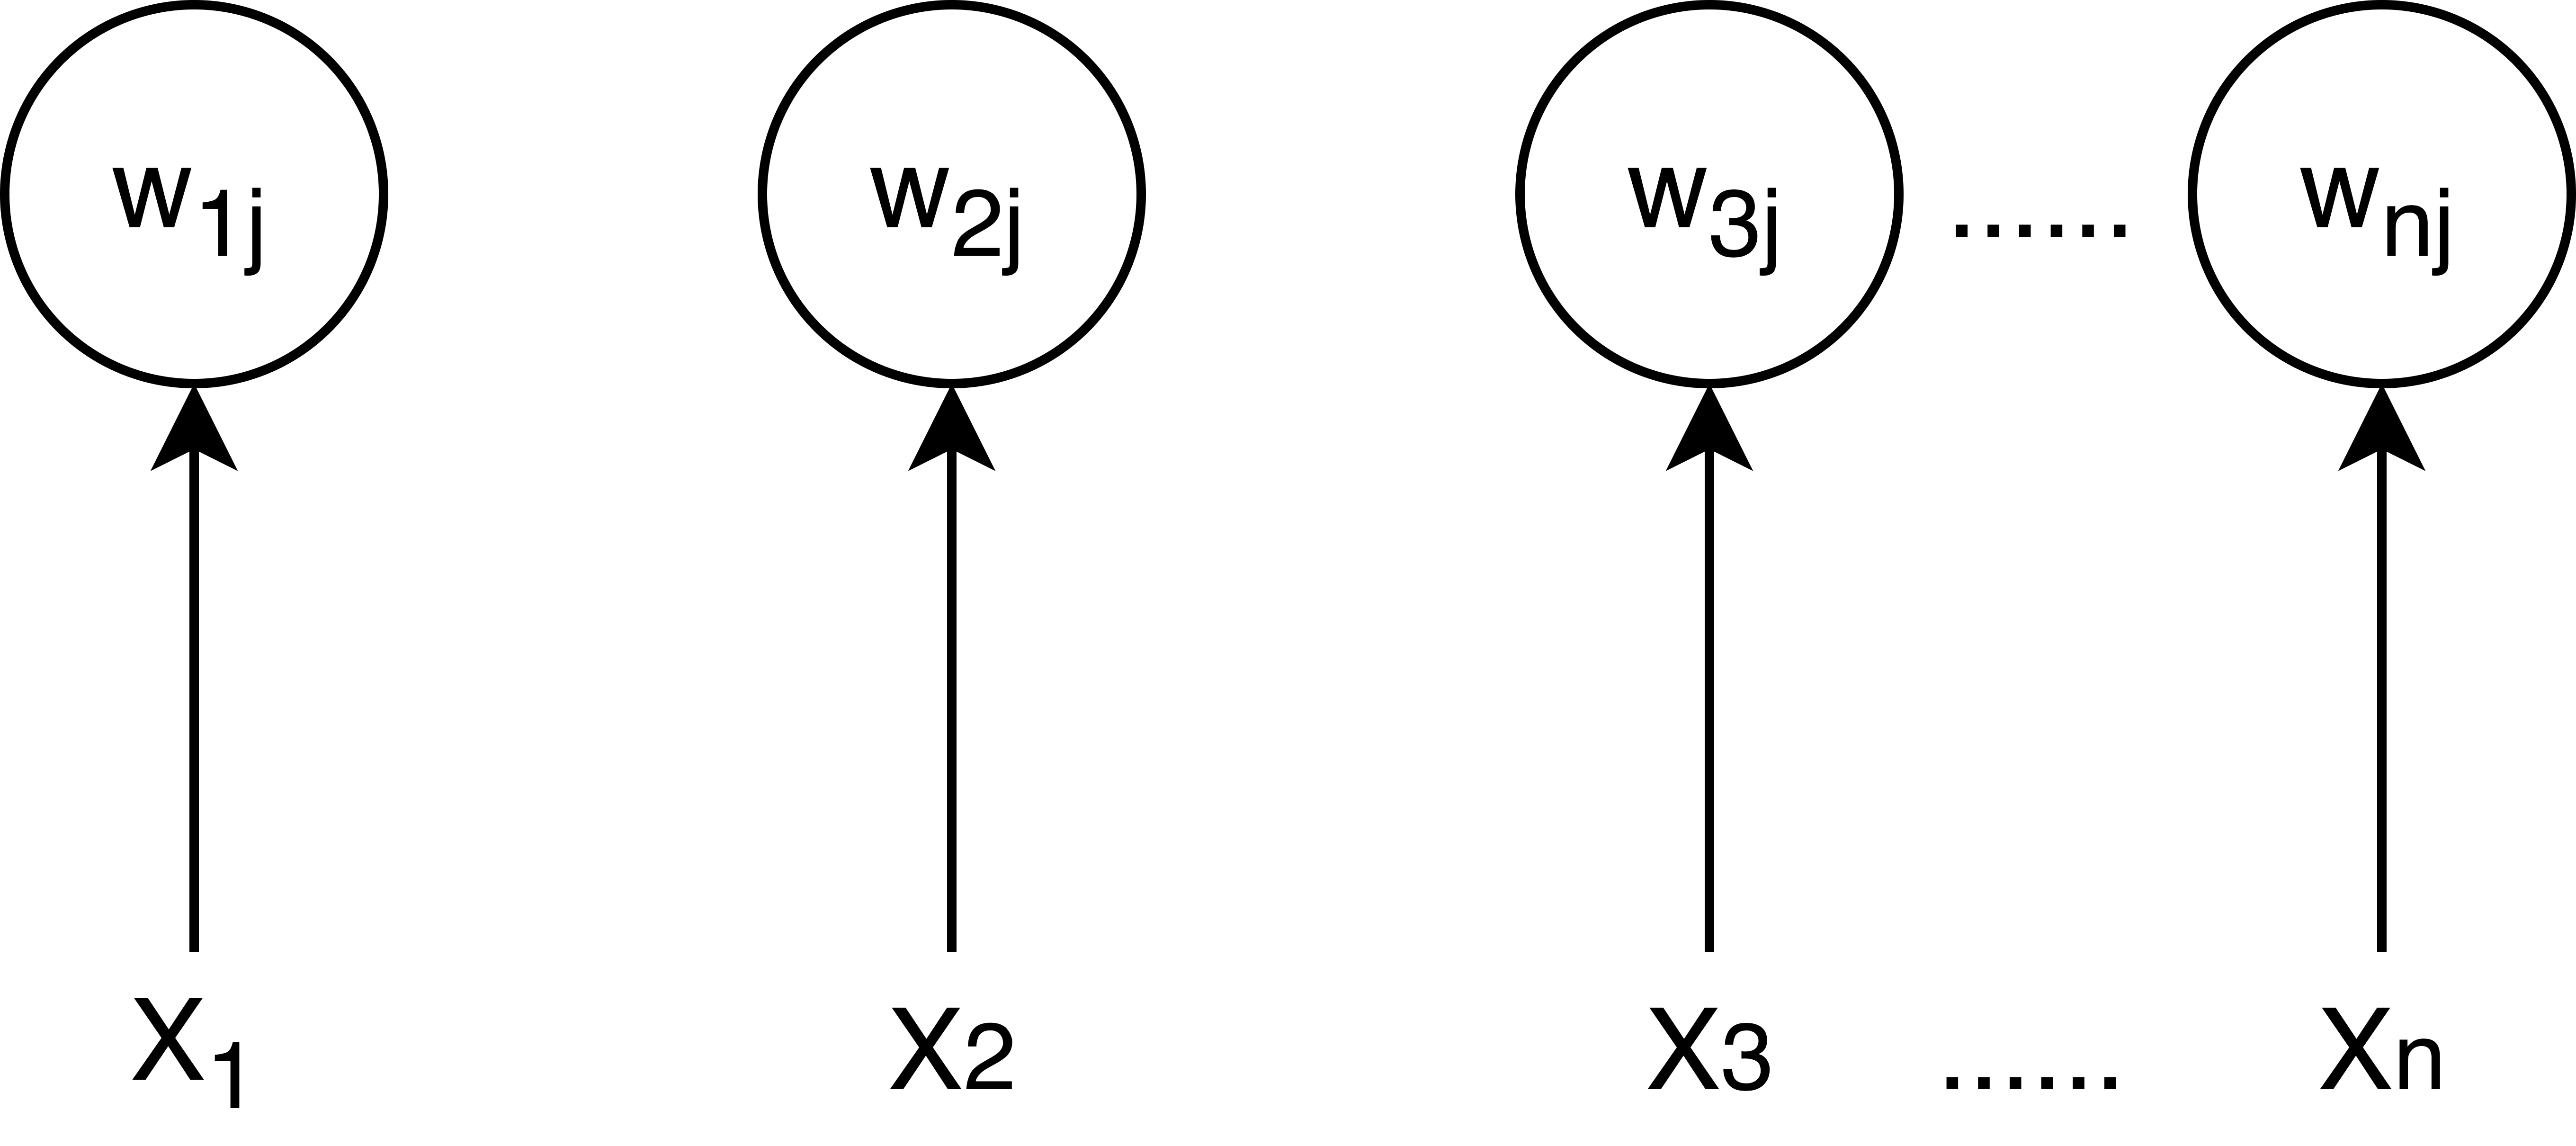
\includegraphics[width=\linewidth, scale = 0.5]{Weights_input_RNN.png}
\caption{Weights between input layer and first hidden layer of neurons} \label{fig:3}
%\end{subfigure}
\end{figure}

%Once we get the input at time step t+n+m+1 (which is ground truth to the prediction of label at X_t+n+m) then we will know the accuracy of the model.


\section{Experimental Setup}

We have used jupyter notebook to write our programs in python language. We have used a keras a Tensorflow backend model for designing our RNNs. 


\begin{algorithm}
\caption{Calculating the time to raise a flag}
\begin{algorithmic}
 \REQUIRE Finding time 't+n+m' at which RNN has to be diagnosed
 \STATE \texttt{\textbf{INPUT}: $Time-series \{X_t, X_t_+_1, ..., X_t_+_n_+_m_+_1\}$}
 \STATE \texttt{\textbf{OUTPUT}: $Time$ $label$ 't+n+m'}
 \STATE $Accuracy \leftarrow Accuracy-prediction\{X_t, X_t_+_1, ..., X_t_+_n_+_m_+_1\}$
 \STATE $Gradients \leftarrow Gradients-prediction\{X_t, X_t_+_1, ..., X_t_+_n_+_m_+_1\}$
     \FOR{Acc in Accuracy and Grad in Gradients:}
         \IF{Acc == min(Acc) and Grad == max(Grad):}
            \STATE \textbf{FLAG}
         \ELSE
             \STATE Continue
    \ENDIF
\ENDFOR
\end{algorithmic}
\end{algorithm}


We have designed an algorithm for knowing accuracy and gradients in post deployment phase. As we can see in Algorithm 1, the input of the algorithm will be unseen stream of time-series data. At each time step 't' RNN will predict the output of the overflow value at 't+1'. Then the accuracy of the prediction is obtained by comparing ground truth value at 't+1' and predicted value at 't'. In the algorithm $Accuracy-prediction \{X_t, X_t+1, ...., X+t+n+m+1\}$ implies the accuracy of predicted values at different time stamps. After each iteration the accuracy at each time step is appended to a bucket called accuracy. $Gradients-prediction \{X_t, X_t+1, ...., X+t+n+m+1\}$ implies the gradient change of the algorithm after each time step. After each iteration the gradient change at each time step is appended to the bucket gradients. The next step of the algorithm shows the automated way of mapping these accuracy values and gradient changes and knowing a particular time stamp 't+n+m' where we have least accuracy ($min(Acc)$) and increase in the gradient descent function ($max(Grad)$). We have considered data points until 't+n+m+1' since the ground truth label of diagnosing time 't+n+m' is at 't+n+m+1'. Only by considering until 't+n+m+1' will we be able to know the accuracy and the gradient change of the model at 't+n+m'.

In Algorithm 1, to gain accuracy values we have calculated the distance between predicted and ground truth values. We can know the accuracy values by using equation (4). It is the mean squared distance between predicted value and the ground truth value. 'n' in this equation is the number of samples predicted until specific time step. By dividing the difference squared with 'n' we will get a mean value of accuracy which when multiplied by 100 will give us a percentage of accuracy of each time stamp.

\begin{equation}
  Accuracy = 1/n * \sqrt{{Ground truth (t+n+1)}^2 - {Predicted (t+n)}^2}
\end{equation}

For obtaining gradients we have used a backend function in keras called $gradients$ and collected all the gradient value at different time stamps. The basic equation of calculating this gradient descent is given in equation (1) and equation (2). After each time stamp the change in gradients $\theta_i$ is calculated by reducing the gradient values at each time step. So when we map this values the graphical representation of this values should have gradual decay in the values. The goal of the algorithm is to find a best converging value of gradients called global minima. Since we cannot have a perfect decaying values for all the time steps we will experience some exponential increase and decrease in the gradient value. In the for loop of Algorithm we have designed in such a way that it will automatically map these changes as the RNN goes on predicting the stream of new datapoints. Our take away point is that at a point where there is a exponential increase in the gradient values and also exponential decay in accuracy values is the point where neural network will lose the capacity to be robust and accurate. 

%%% Insert Table showing layers of the RNN like input having 128 neurons two hidden layers and output with sigmoid activation


%%%Give table showing accuracies of pre-deployment%%%
\subsection{LSTM}
Long short term memory is a variant of RNN where the 
%write about LSTM, GRU, Ind RNN in detail. Then write about the python, jupyter notebook, Number of neurons chosen in each variant of RNN in a tabular form

The title of your work should use capital letters appropriately -
\url{https://capitalizemytitle.com/} has useful rules for
capitalization. Use the {\verb|title|} command to define the title of
your work. If your work has a subtitle, define it with the
{\verb|subtitle|} command.  Do not insert line breaks in your title.

If your title is lengthy, you must define a short version to be used
in the page headers, to prevent overlapping text. The \verb|title|
command has a ``short title'' parameter:
\begin{verbatim}
  \title[short title]{full title}
\end{verbatim}

\section{Authors and Affiliations}

Each author must be defined separately for accurate metadata
identification. Multiple authors may share one affiliation. Authors'
names should not be abbreviated; use full first names wherever
possible. Include authors' e-mail addresses whenever possible.

Grouping authors' names or e-mail addresses, or providing an ``e-mail
alias,'' as shown below, is not acceptable:
\begin{verbatim}
  \author{Brooke Aster, David Mehldau}
  \email{dave,judy,steve@university.edu}
  \email{firstname.lastname@phillips.org}
\end{verbatim}

The \verb|authornote| and \verb|authornotemark| commands allow a note
to apply to multiple authors --- for example, if the first two authors
of an article contributed equally to the work.

If your author list is lengthy, you must define a shortened version of
the list of authors to be used in the page headers, to prevent
overlapping text. The following command should be placed just after
the last \verb|\author{}| definition:
\begin{verbatim}
  \renewcommand{\shortauthors}{McCartney, et al.}
\end{verbatim}
Omitting this command will force the use of a concatenated list of all
of the authors' names, which may result in overlapping text in the
page headers.

The article template's documentation, available at
\url{https://www.acm.org/publications/proceedings-template}, has a
complete explanation of these commands and tips for their effective
use.

Note that authors' addresses are mandatory for journal articles.

\section{Rights Information}

Authors of any work published by ACM will need to complete a rights
form. Depending on the kind of work, and the rights management choice
made by the author, this may be copyright transfer, permission,
license, or an OA (open access) agreement.

Regardless of the rights management choice, the author will receive a
copy of the completed rights form once it has been submitted. This
form contains \LaTeX\ commands that must be copied into the source
document. When the document source is compiled, these commands and
their parameters add formatted text to several areas of the final
document:
\begin{itemize}
\item the ``ACM Reference Format'' text on the first page.
\item the ``rights management'' text on the first page.
\item the conference information in the page header(s).
\end{itemize}

Rights information is unique to the work; if you are preparing several
works for an event, make sure to use the correct set of commands with
each of the works.

The ACM Reference Format text is required for all articles over one
page in length, and is optional for one-page articles (abstracts).

\section{CCS Concepts and User-Defined Keywords}

Two elements of the ``acmart'' document class provide powerful
taxonomic tools for you to help readers find your work in an online
search.

The ACM Computing Classification System ---
\url{https://www.acm.org/publications/class-2012} --- is a set of
classifiers and concepts that describe the computing
discipline. Authors can select entries from this classification
system, via \url{https://dl.acm.org/ccs/ccs.cfm}, and generate the
commands to be included in the \LaTeX\ source.

User-defined keywords are a comma-separated list of words and phrases
of the authors' choosing, providing a more flexible way of describing
the research being presented.

CCS concepts and user-defined keywords are required for for all
articles over two pages in length, and are optional for one- and
two-page articles (or abstracts).

\section{Sectioning Commands}

Your work should use standard \LaTeX\ sectioning commands:
\verb|section|, \verb|subsection|, \verb|subsubsection|, and
\verb|paragraph|. They should be numbered; do not remove the numbering
from the commands.

Simulating a sectioning command by setting the first word or words of
a paragraph in boldface or italicized text is {\bfseries not allowed.}

\section{Tables}

The ``\verb|acmart|'' document class includes the ``\verb|booktabs|''
package --- \url{https://ctan.org/pkg/booktabs} --- for preparing
high-quality tables.

Table captions are placed {\itshape above} the table.

Because tables cannot be split across pages, the best placement for
them is typically the top of the page nearest their initial cite.  To
ensure this proper ``floating'' placement of tables, use the
environment \textbf{table} to enclose the table's contents and the
table caption.  The contents of the table itself must go in the
\textbf{tabular} environment, to be aligned properly in rows and
columns, with the desired horizontal and vertical rules.  Again,
detailed instructions on \textbf{tabular} material are found in the
\textit{\LaTeX\ User's Guide}.

Immediately following this sentence is the point at which
Table~\ref{tab:freq} is included in the input file; compare the
placement of the table here with the table in the printed output of
this document.

\begin{table}
  \caption{Frequency of Special Characters}
  \label{tab:freq}
  \begin{tabular}{ccl}
    \toprule
    Non-English or Math&Frequency&Comments\\
    \midrule
    \O & 1 in 1,000& For Swedish names\\
    $\pi$ & 1 in 5& Common in math\\
    \$ & 4 in 5 & Used in business\\
    $\Psi^2_1$ & 1 in 40,000& Unexplained usage\\
  \bottomrule
\end{tabular}
\end{table}

To set a wider table, which takes up the whole width of the page's
live area, use the environment \textbf{table*} to enclose the table's
contents and the table caption.  As with a single-column table, this
wide table will ``float'' to a location deemed more
desirable. Immediately following this sentence is the point at which
Table~\ref{tab:commands} is included in the input file; again, it is
instructive to compare the placement of the table here with the table
in the printed output of this document.

\begin{table*}
  \caption{Some Typical Commands}
  \label{tab:commands}
  \begin{tabular}{ccl}
    \toprule
    Command &A Number & Comments\\
    \midrule
    \texttt{{\char'134}author} & 100& Author \\
    \texttt{{\char'134}table}& 300 & For tables\\
    \texttt{{\char'134}table*}& 400& For wider tables\\
    \bottomrule
  \end{tabular}
\end{table*}

\section{Math Equations}
You may want to display math equations in three distinct styles:
inline, numbered or non-numbered display.  Each of the three are
discussed in the next sections.

\subsection{Inline (In-text) Equations}
A formula that appears in the running text is called an inline or
in-text formula.  It is produced by the \textbf{math} environment,
which can be invoked with the usual
\texttt{{\char'134}begin\,\ldots{\char'134}end} construction or with
the short form \texttt{\$\,\ldots\$}. You can use any of the symbols
and structures, from $\alpha$ to $\omega$, available in
\LaTeX~\cite{Lamport:LaTeX}; this section will simply show a few
examples of in-text equations in context. Notice how this equation:
\begin{math}
  \lim_{n\rightarrow \infty}x=0
\end{math},
set here in in-line math style, looks slightly different when
set in display style.  (See next section).

\subsection{Display Equations}
A numbered display equation---one set off by vertical space from the
text and centered horizontally---is produced by the \textbf{equation}
environment. An unnumbered display equation is produced by the
\textbf{displaymath} environment.

Again, in either environment, you can use any of the symbols and
structures available in \LaTeX\@; this section will just give a couple
of examples of display equations in context.  First, consider the
equation, shown as an inline equation above:
\begin{equation}
  \lim_{n\rightarrow \infty}x=0
\end{equation}
Notice how it is formatted somewhat differently in
the \textbf{displaymath}
environment.  Now, we'll enter an unnumbered equation:
\begin{displaymath}
  \sum_{i=0}^{\infty} x + 1
\end{displaymath}
and follow it with another numbered equation:
\begin{equation}
  \sum_{i=0}^{\infty}x_i=\int_{0}^{\pi+2} f
\end{equation}
just to demonstrate \LaTeX's able handling of numbering.

%\section{Figures}

The ``\verb|figure|'' environment should be used for figures. One or
more images can be placed within a figure. If your figure contains
third-party material, you must clearly identify it as such, as shown
in the example below.


%\usepackage{subcaption}
%\usepackage[demo]{graphicx} % omit 'demo' for real document
\begin{figure*}
%\begin{subfigure}{\textwidth}
\includegraphics[width= 6in]{Post-Deployment.png}
\caption{Figure shows the working of RNN post-deployment and how our algorithms flags at a particular time (t+n+m) inferring the time to repair RNN} \label{fig:4}
%\end{subfigure}
\end{figure*}
Your figures should contain a caption which describes the figure to
the reader. Figure captions go below the figure. Your figures should
{\bfseries also} include a description suitable for screen readers, to
assist the visually-challenged to better understand your work.

Figure captions are placed {\itshape below} the figure.

\subsection{The ``Teaser Figure''}

A ``teaser figure'' is an image, or set of images in one figure, that
are placed after all author and affiliation information, and before
the body of the article, spanning the page. If you wish to have such a
figure in your article, place the command immediately before the
\verb|\maketitle| command:
\begin{verbatim}
  \begin{teaserfigure}
    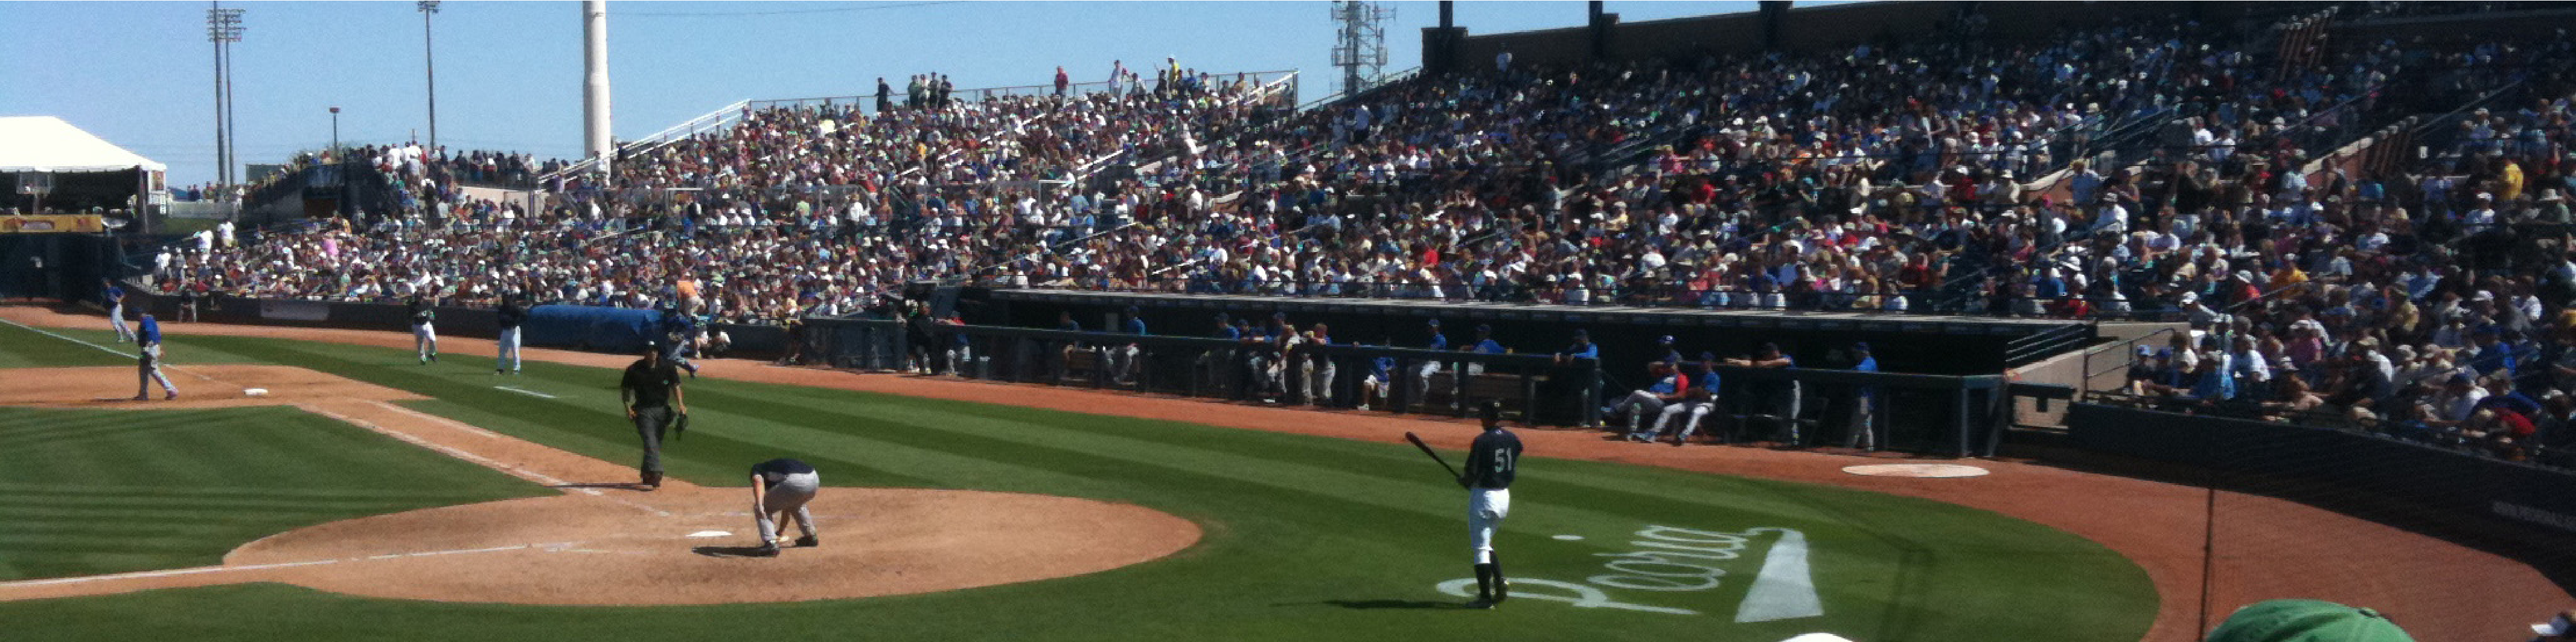
\includegraphics[width=\textwidth]{sampleteaser}
    \caption{figure caption}
    \Description{figure description}
  \end{teaserfigure}
\end{verbatim}

\section{Citations and Bibliographies}

The use of \BibTeX\ for the preparation and formatting of one's
references is strongly recommended. Authors' names should be complete
--- use full first names (``Donald E. Knuth'') not initials
(``D. E. Knuth'') --- and the salient identifying features of a
reference should be included: title, year, volume, number, pages,
article DOI, etc.

The bibliography is included in your source document with these two
commands, placed just before the \verb|\end{document}| command:
\begin{verbatim}
  \bibliographystyle{ACM-Reference-Format}
  \bibliography{bibfile}
\end{verbatim}
where ``\verb|bibfile|'' is the name, without the ``\verb|.bib|''
suffix, of the \BibTeX\ file.

Citations and references are numbered by default. A small number of
ACM publications have citations and references formatted in the
``author year'' style; for these exceptions, please include this
command in the {\bfseries preamble} (before
``\verb|\begin{document}|'') of your \LaTeX\ source:
\begin{verbatim}
  \citestyle{acmauthoryear}
\end{verbatim}

  Some examples.  A paginated journal article \cite{Abril07}, an
  enumerated journal article \cite{Cohen07}, a reference to an entire
  issue \cite{JCohen96}, a monograph (whole book) \cite{Kosiur01}, a
  monograph/whole book in a series (see 2a in spec. document)
  \cite{Harel79}, a divisible-book such as an anthology or compilation
  \cite{Editor00} followed by the same example, however we only output
  the series if the volume number is given \cite{Editor00a} (so
  Editor00a's series should NOT be present since it has no vol. no.),
  a chapter in a divisible book \cite{Spector90}, a chapter in a
  divisible book in a series \cite{Douglass98}, a multi-volume work as
  book \cite{Knuth97}, an article in a proceedings (of a conference,
  symposium, workshop for example) (paginated proceedings article)
  \cite{Andler79}, a proceedings article with all possible elements
  \cite{Smith10}, an example of an enumerated proceedings article
  \cite{VanGundy07}, an informally published work \cite{Harel78}, a
  doctoral dissertation \cite{Clarkson85}, a master's thesis:
  \cite{anisi03}, an online document / world wide web resource
  \cite{Thornburg01, Ablamowicz07, Poker06}, a video game (Case 1)
  \cite{Obama08} and (Case 2) \cite{Novak03} and \cite{Lee05} and
  (Case 3) a patent \cite{JoeScientist001}, work accepted for
  publication \cite{rous08}, 'YYYYb'-test for prolific author
  \cite{SaeediMEJ10} and \cite{SaeediJETC10}. Other cites might
  contain 'duplicate' DOI and URLs (some SIAM articles)
  \cite{Kirschmer:2010:AEI:1958016.1958018}. Boris / Barbara Beeton:
  multi-volume works as books \cite{MR781536} and \cite{MR781537}. A
  couple of citations with DOIs:
  \cite{2004:ITE:1009386.1010128,Kirschmer:2010:AEI:1958016.1958018}. Online
  citations: \cite{TUGInstmem, Thornburg01, CTANacmart}. Artifacts:
  \cite{R} and \cite{UMassCitations}.

\section{Acknowledgments}

Identification of funding sources and other support, and thanks to
individuals and groups that assisted in the research and the
preparation of the work should be included in an acknowledgment
section, which is placed just before the reference section in your
document.

This section has a special environment:
\begin{verbatim}
  \begin{acks}
  ...
  \end{acks}
\end{verbatim}
so that the information contained therein can be more easily collected
during the article metadata extraction phase, and to ensure
consistency in the spelling of the section heading.

Authors should not prepare this section as a numbered or unnumbered {\verb|\section|}; please use the ``{\verb|acks|}'' environment.

\section{Appendices}

If your work needs an appendix, add it before the
``\verb|\end{document}|'' command at the conclusion of your source
document.

Start the appendix with the ``\verb|appendix|'' command:
\begin{verbatim}
  \appendix
\end{verbatim}
and note that in the appendix, sections are lettered, not
numbered. This document has two appendices, demonstrating the section
and subsection identification method.

\section{SIGCHI Extended Abstracts}

The ``\verb|sigchi-a|'' template style (available only in \LaTeX\ and
not in Word) produces a landscape-orientation formatted article, with
a wide left margin. Three environments are available for use with the
``\verb|sigchi-a|'' template style, and produce formatted output in
the margin:
\begin{itemize}
\item {\verb|sidebar|}:  Place formatted text in the margin.
\item {\verb|marginfigure|}: Place a figure in the margin.
\item {\verb|margintable|}: Place a table in the margin.
\end{itemize}

%%
%% The acknowledgments section is defined using the "acks" environment
%% (and NOT an unnumbered section). This ensures the proper
%% identification of the section in the article metadata, and the
%% consistent spelling of the heading.
\begin{acks}
To Robert, for the bagels and explaining CMYK and color spaces.
\end{acks}

%%
%% The next two lines define the bibliography style to be used, and
%% the bibliography file.
\bibliographystyle{ACM-Reference-Format}
\bibliography{sample-base}

%%
%% If your work has an appendix, this is the place to put it.
\appendix

\section{Research Methods}

\subsection{Part One}

Lorem ipsum dolor sit amet, consectetur adipiscing elit. Morbi
malesuada, quam in pulvinar varius, metus nunc fermentum urna, id
sollicitudin purus odio sit amet enim. Aliquam ullamcorper eu ipsum
vel mollis. Curabitur quis dictum nisl. Phasellus vel semper risus, et
lacinia dolor. Integer ultricies commodo sem nec semper.

\subsection{Part Two}

Etiam commodo feugiat nisl pulvinar pellentesque. Etiam auctor sodales
ligula, non varius nibh pulvinar semper. Suspendisse nec lectus non
ipsum convallis congue hendrerit vitae sapien. Donec at laoreet
eros. Vivamus non purus placerat, scelerisque diam eu, cursus
ante. Etiam aliquam tortor auctor efficitur mattis.

\section{Online Resources}

Nam id fermentum dui. Suspendisse sagittis tortor a nulla mollis, in
pulvinar ex pretium. Sed interdum orci quis metus euismod, et sagittis
enim maximus. Vestibulum gravida massa ut felis suscipit
congue. Quisque mattis elit a risus ultrices commodo venenatis eget
dui. Etiam sagittis eleifend elementum.

Nam interdum magna at lectus dignissim, ac dignissim lorem
rhoncus. Maecenas eu arcu ac neque placerat aliquam. Nunc pulvinar
massa et mattis lacinia.

\end{document}
\endinput
%%
%% End of file `sample-sigconf.tex'.
